\documentclass[12pt]{article}
\usepackage{geometry}
\geometry{a4paper}

\usepackage[parfill]{parskip}    % Activate to begin paragraphs with an empty line rather than an indent
\usepackage{graphicx}
\usepackage{amssymb}
\usepackage{epstopdf}
\usepackage{fancyhdr}
\usepackage{fullpage}
\usepackage{appendix}
\usepackage{newclude}
\usepackage{datetime}
\usepackage{hyperref}
\usepackage{color}
\usepackage{multicol}
\usepackage{tabularx}
\usepackage{enumerate}
\usepackage{enumitem}
\usepackage{listings}
\usepackage{wallpaper}
\usepackage{lastpage}
\usepackage{titling}
\usepackage{multind}
\usepackage[table]{xcolor}
\usepackage{mathtools}
\usepackage{tikz}
\usepackage{longtable}
\usepackage[section]{placeins}
%\geometry{landscape}
\usetikzlibrary{shapes,arrows}

\tikzstyle{block} = [rectangle, draw, text width = 6em, text centered, rounded corners, minimum height = 4em]
\tikzstyle{inputblock} = [rectangle, draw, text width = 24em, minimum height = 2.5em]
\tikzstyle{autographblock} = [rectangle, draw, fill = black!1, text height = 0, text depth = 2cm,text width = 24em, minimum height = 8em]
\tikzstyle{cloud} = [ellipse, draw, minimum height = 4em]
\tikzstyle{line} = [draw, -latex']

\makeindex{modules}


\newcommand{\usemodule}[1]{\index{modules}{#1}\texttt{#1}}

\definecolor{gray}{rgb}{0.5,0.5,0.5}
\definecolor{tableheader}{rgb}{0.7,0.7,0.7}

\setlist[description]{style=nextline}
\renewcommand{\familydefault}{\sfdefault}

% link setup
\hypersetup{
    colorlinks,
    citecolor=black,
    filecolor=black,
    linkcolor=black,
    urlcolor=black,
}

\DeclareGraphicsRule{.tif}{png}{.png}{`convert #1 `dirname #1`/`basename #1 .tif`.png}

% usefull commands:
\newcommand{\seeref}[1]{\ref{#1} p.\pageref{#1}}
%\newcommand{\see}[1]{ (zie \ref{#1} p.\pageref{#1})}
\newcommand{\seesee}[2]{ (zie \ref{#1} p.\pageref{#1},  \ref{#2} p.\pageref{#2})}

% style for code blocks
\lstset{
    linewidth=1\textwidth,
    breaklines=true,
    numbers=left,                   % where to put the line-numbers
    numberstyle=\tiny\color{gray},  % the style that is used for the line-numbers
    stepnumber=1,                   % the step between two line-numbers. If it's 1, each line 
    numbersep=5pt, 
    basicstyle=\footnotesize,
}

% Header and Footer settings
\URCornerWallPaper{0.13}{img/dop/koptekstlogo.png}
\pagestyle{fancy}
\fancyhead{}
\renewcommand{\headrulewidth}{0pt}

% Settings for table of contents.   
\setcounter{secnumdepth}{4}
\setcounter{tocdepth}{3}

\makeatletter
% some extra spacing for the table of contents
\renewcommand{\l@subsection}{\@dottedtocline{2}{1.5em}{3em}}
\renewcommand{\l@subsubsection}{\@dottedtocline{2}{2.7em}{4em}}

\renewcommand\paragraph{%
   \@startsection{paragraph}{4}{0mm}%
      {-\baselineskip}%
      {.5\baselineskip}%
      {\normalfont\normalsize\bfseries}}
\makeatother

\renewcommand{\dateseparator}{-}
\renewcommand{\figurename}{Figuur}

% Define variables
\newcommand{\customer}{Dimpact}
\newcommand{\projectname}{Dimpact}
\newcommand{\thecustomer}{\customer }
\newcommand{\customerdomain}{dimpact.nl}
\newcommand{\customerdomainfull}{http://www.dimpact.nl}
\newcommand{\customerdomainuc}{Dimpact.nl}
\newcommand{\authors}{David van Dijk \\ & Patrick Kraaij }
\newcommand{\version}{0.1}

\fancyfoot[L]{Functioneel ontwerp - \customer}
\fancyfoot[C]{v\version \ \ddmmyyyydate \today}
\fancyfoot[R]{\textbf{\thepage}\ / \pageref{LastPage}}

\title{\textbf{\customerdomainuc} \\ Functioneel Ontwerp}
\pretitle{\begin{flushleft}\LARGE}
\posttitle{\par\end{flushleft}}

\author{}  % skippen we voor maketitle
\date{}

% The actual Document:
\begin{document}
\ThisLRCornerWallPaper{0.8}{img/dop/voorbladlogo.png}

  \maketitle
 \vspace{-2.6cm}
  \begin{flushright}
\begin{tabularx}{4.6cm}{ X }
Dutch Open Projects         \\
Doornseweg 12                   \\  
3832 RL Leusden                 \\
T: +31[0]33 - 4 50 50 50        \\
F: +31[0]33 - 4 50 50 57        
\\*
\\*
\\*
\\*
\\*
\\*
\\*
\\*
\\*
\\*
\\*
\\*
\\*
\\*
\\*
\\*
\\*
\\*
\\*
\\*



\footnotesize
\copyright All rights reserved.         \\*
\footnotesize
No part of the contents of this publication may be reproduced, stored in a data processing system or transmitted in any form or by any means without the written permission of Dutch Open Projects B.V.

\end{tabularx}
\end{flushright}

\begin{tabularx}{\linewidth}{ p{3cm} X }
  Plaats & Leusden                                \\
  Laatst bijgewerkt & \ddmmyyyydate \today        \\
  Auteurs & \authors                          \\
  Versie & \version                                    \\
\end{tabularx}
\pagebreak




\pagebreak
\subsection*{Akkoord}
Voor akkoord:\\ \\
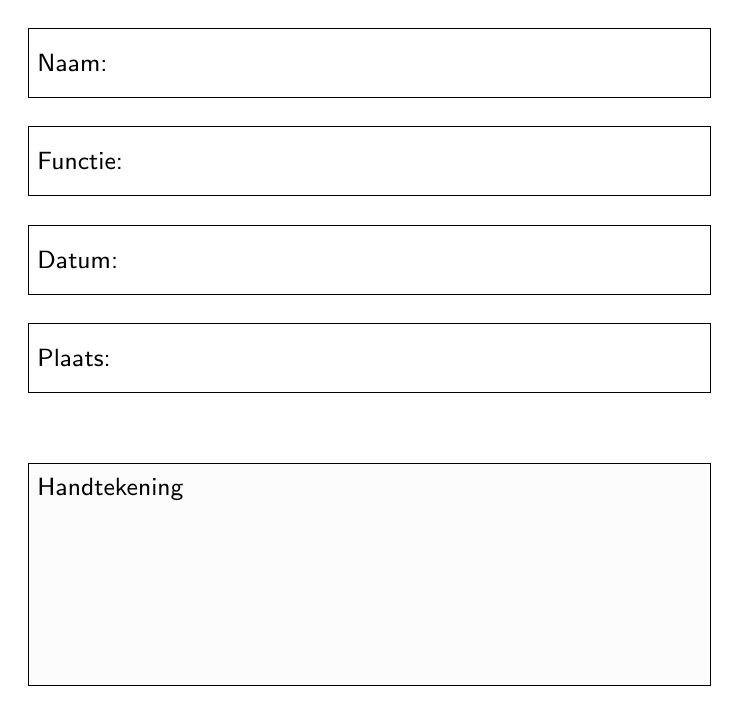
\begin{tikzpicture}
\tikzstyle{every node}=[font=\small];
\node [inputblock] (names) {Naam:};
\node [inputblock, below of = names, node distance = 1.25cm] (function) {Functie:};
\node [inputblock, below of = function, node distance = 1.25cm] (dates) {Datum:};
\node [inputblock, below of = dates, node distance = 1.25cm] (place) {Plaats:};
\node [autographblock, below of = place, node distance = 2.75cm] (autograph) {Handtekening};
\end{tikzpicture}
\pagebreak

% table of contents
\renewcommand*\contentsname{Inhoudsopgave}
\tableofcontents

\pagebreak


\section{Introductie}

\subsection{Management summary}
In het document Technisch Ontwerp \customerdomain \ wordt de technische implementatie beschreven. Het is een blauwdruk voor ontwikkelaars. 

\subsection{Opbouw document}
Dit document dient als leidraad voor de bouw van dit project. Het belangrijkste onderdeel ervan zijn daarom de componenten\seeone{componenten}. Componenten bieden een opsplitsing van de functionaliteiten binnen de website, zowel zichtbaar als niet zichtbaar. Tijdens de bouw zal een ontwikkelaar aan \'{e}\'{e}n specifiek component tegelijk werken. Daarnaast worden in dit document een aantal randzaken zoals deployment\seeone{deployment} en performance\seeone{performance} en algemene eisen\seeone{algemeen} beschreven in eerdere hoofdstukken. In de appendix vindt met een overzicht van Drupal specifieke zaken zoals content types en views, maar ook referentietabellen die aangeven waar welk onderdeel uit het interactieontwerp\seeone{ioto} of de design briefing\seeone{dbto} is beschreven.

\section{Pagina's}
\label{sec:paginas}

Hieronder worden alle pagina's opgesomd die zijn gemaakt in het wireframe. Per pagina worden alle blokken opgesomd. De volgende componenten komen voor op alle pagina's.
\begin{itemize}
  \item Logo en naam zie \ref{sec:logoennaam}
  \item Meta menu \ref{sec:metamenu}
  \item Tabs \ref{sec:tabspagina}
  \item Hoofdnavigatie \ref{sec:hoofdnavigatie}
  \item Zoekveld \ref{sec:zoekveld}
  \item Alfabetische balk \ref{sec:alfabetischebalk}
  \item Vrije HTML Footer \ref{sec:vrijehtmlfooter}
  \item DigiD \ref{sec:digid}
\end{itemize}

\subsection{Regios}
\label{sec:regios}

\begin{center}
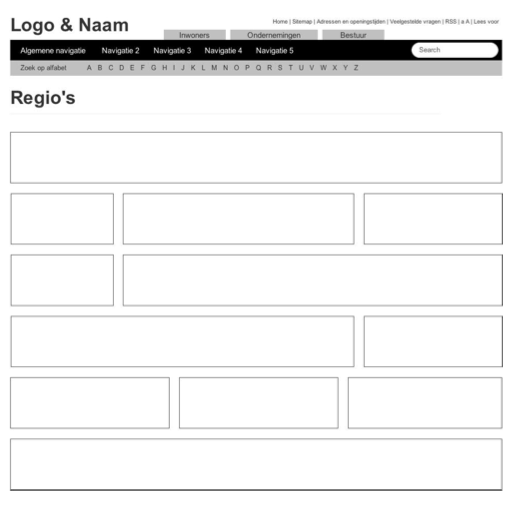
\includegraphics[scale=.5]{img/regions.png}
\end{center}

Op de pagina zijn de volgende regio's gedefinieerd. Aan de boven- en onderkant van de pagina zijn regio's over de hele breedte van de pagina beschikbaar. Daarnaast kent de template de volgende opstellingen.

\begin{description}
\item[Drie kolommen - smal / breed / smal] Deze opzet bestaat uit drie regio's waarbij de linker en rechter smaller zijn dan de middelste regio.
\item[Twee kolommen - smal / breed] Deze opzet bestaat uit twee regio's waarbij de linker regio smaller is dan de rechter.
\item[Twee kolommen - breed / smal] Deze opzet bestaat uit twee regio's waarbij de linker regio breder is dan de rechter.
\item[Drie kolommen] Deze opzet bestaat uit drie regio's die allen even breed zijn.
\end{description}

\subsection{Voorpagina}\label{voorpagina}

\subsubsection{Grid}

De template van de website bestaat uit een grid, een soort geraamte. Het grid is opgebouwd uit verschillende regio's. In elke regio kunnen blokken geplaatst worden. In de paragraaf \emph{Felix}\seeone{felix} staat beschreven hoe en welke je blokken kunt toevoegen aan een regio. 

\bigskip

\begin{center}
	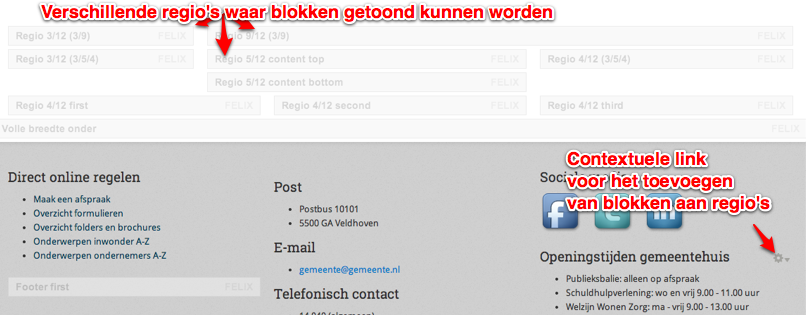
\includegraphics[width=\textwidth]{img/grid1.png}
\end{center}

\subsubsection{Blokken}

In het onderstaande afbeelding worden alle bestaande blokken op voorpagina in het kort toegelicht.

\bigskip

\begin{center}
	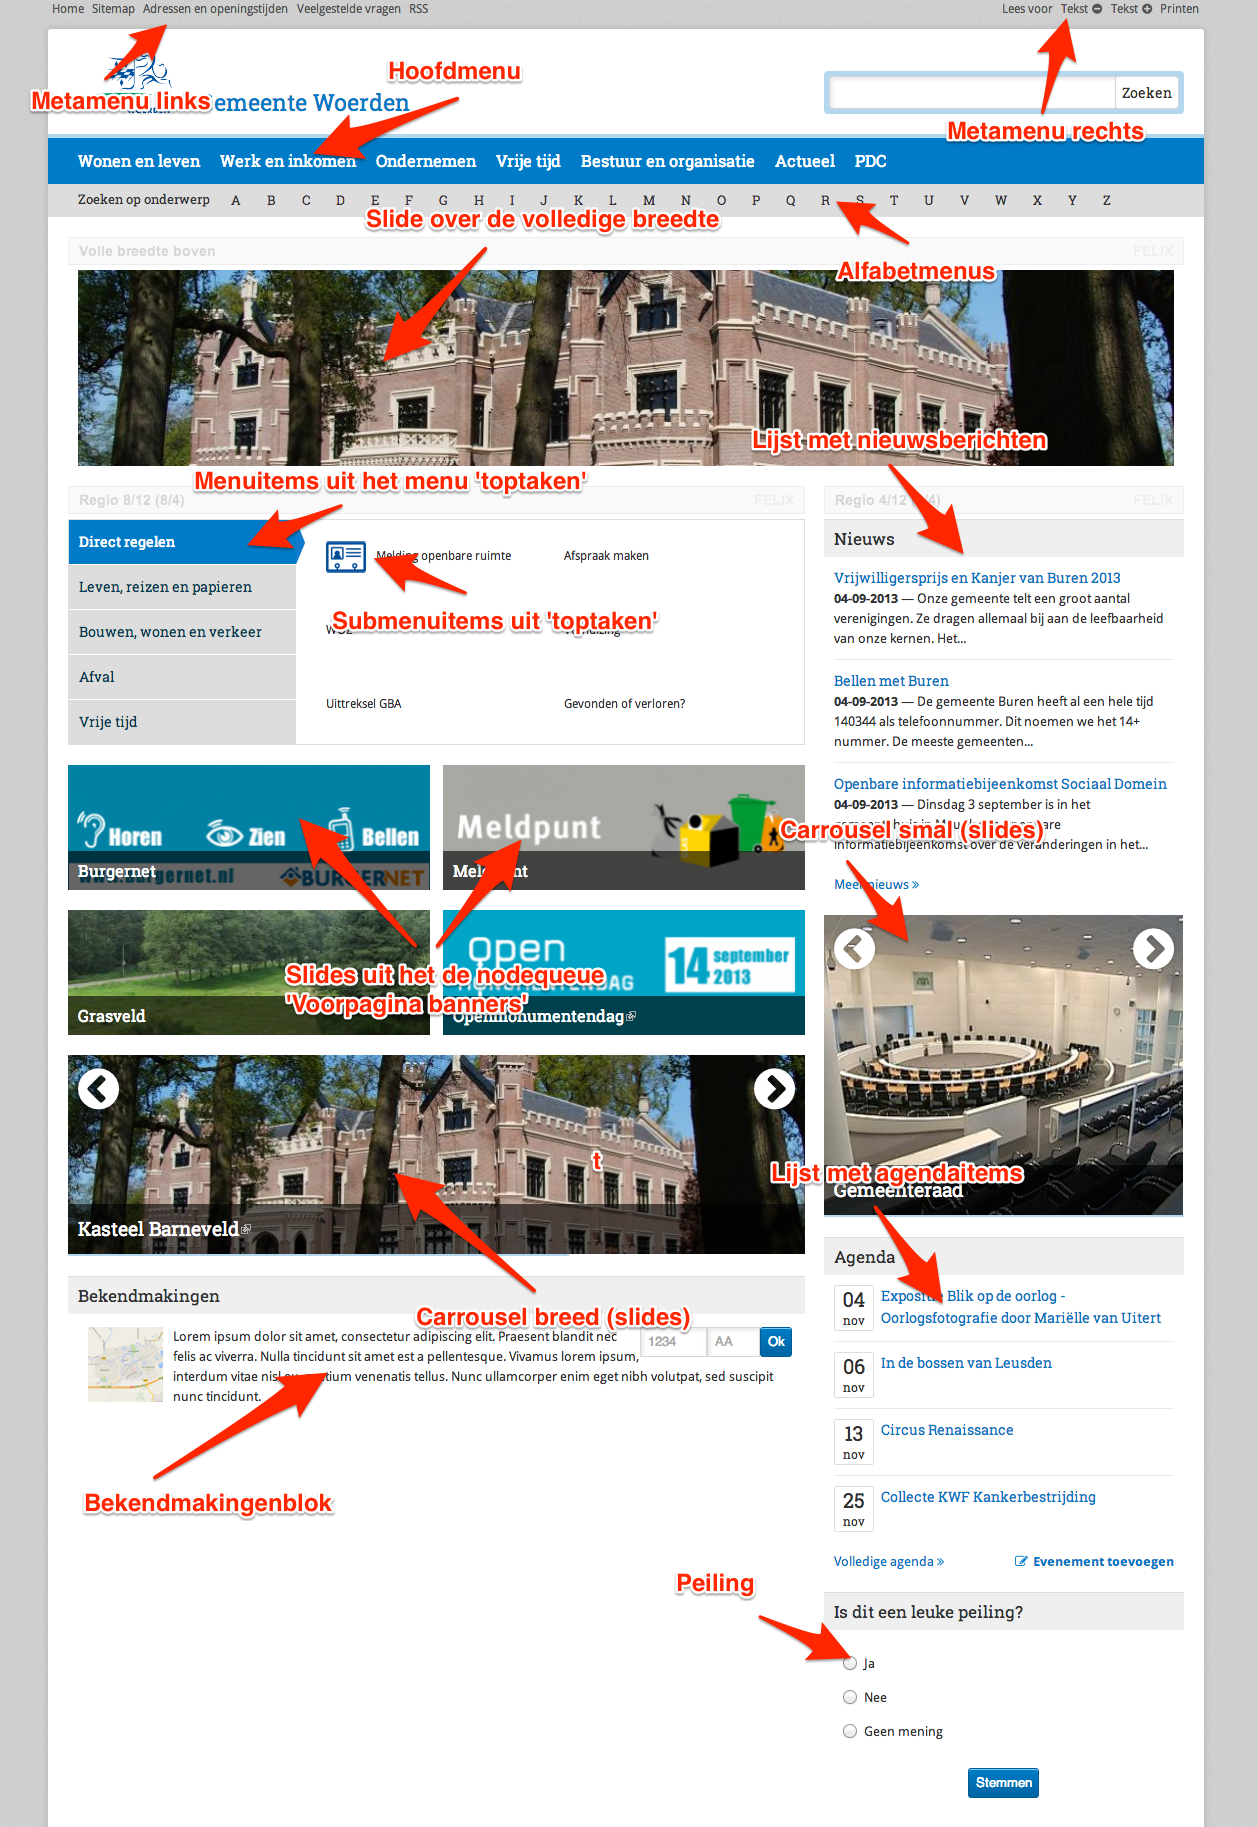
\includegraphics[width=\textwidth]{img/voorpagina.png}
\end{center}

\subsubsection{Footer}

In het onderstaande afbeelding worden alle bestaande blokken in de footer in het kort toegelicht. De footer bestaat uit 3 regio's waar blokken in gezet kunnen worden. De standaard configuratie is links een menu blok "Direct online regelen", in het hoofdstuk \emph{Menu}\seeone{menu} wordt beschreven hoe het menu te bewerken is. In de middenkolom staat blok met redactionele content. In de rechterkolom staan twee blokken; het eerste blok is het Dominion social blok. In paragraaf \emph{Social media}\seeone{socialmedia} staat beschreven hoe deze opties te beheren zijn. Daaronder staat nog een blok met redactionele content. Naast de standaard geconfigureerde blokken zijn in de drie regio's ook nog Felix blokken te zetten. 

\bigskip

\begin{center}
	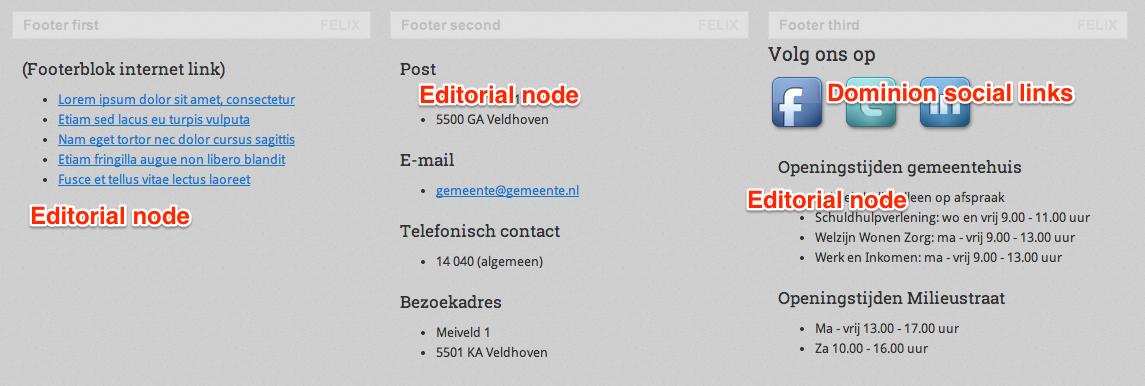
\includegraphics[width=\textwidth]{img/voorpagina3.png}
\end{center}
\subsection{Sub homepagina}
\label{sec:subhomepagina}
\subsection{Lijstpagina}
\label{sec:lijstpagina}
\subsection{Detail- en infopagina}
\label{sec:detaileninfopagina}

\begin{itemize}
  \item Agendalijstblok zie \ref{sec:agendalijst}
  \item Menublok hierarchisch zie \ref{sec:menublokhierarchisch}
  \item Gerelateerde items blok zie \ref{sec:gerelateerdeitems}
\end{itemize}

\subsubsection{Tabs}
\label{sec:detaileninfopaginatabs}

\begin{itemize}
  \item Agendalijstblok zie \ref{sec:agendalijst}
  \item Menublok hierarchisch zie \ref{sec:menublokhierarchisch}
  \item Gerelateerde items blok zie \ref{sec:gerelateerdeitems}
\end{itemize}

\subsection{Zoekresultaten}
\label{sec:zoekresultaten}
\subsection{Bekendmakingen}\label{bekendmakingen}

Bekendmakingen worden opgeslagen als Drupal nodes. Deze worden ge\"{i}mporteerd uit GVOP.

\subsubsection{Kaart en lijstweergave}\label{bekendmakingen-op-de-kaart}

De kaart wordt ontwikkeld m.b.v. views. Zie \seeref{bekendmakingen-markers}. De tekstuele resultaten worden middels een attachment bij deze view ingeladen \seeref{bekendmakingen-overzicht}.

De kaart wordt gemaakt met de \usemodule{gmap} module i.c.m. \usemodule{views}. Via \emph{exposed filters} wordt de volgende filtering aangeboden (in een apart blok):
\begin{itemize}
\item Zoeken op titel
\item Datum (van / tot)
\item Postcode (alleen exacte matching)
\item Status aanvraag (taxonomie, via checkboxes)
\end{itemize}
De filtering heeft zowel invloed op de kaart als op de lijst onder de kaart.


\subsection{Agenda}
\label{sec:agenda}

\begin{itemize}
  \item Tabsblok met nieuws en agenda zie \ref{sec:tabsmetnieuwsenagenda}
  \item Menublok hierarchisch zie \ref{sec:menublokhierarchisch}
  \item Gerelateerde items blok zie \ref{sec:gerelateerdeitems}
  \item Google Maps blok zie \ref{sec:maps}  
\end{itemize}

\subsection{Pagina met inhoudsopgave}
\label{sec:paginametinhoudsopgave}

\begin{itemize}
  \item Agendalijstblok zie \ref{sec:agendalijst}
  \item Menublok hierarchisch zie \ref{sec:menublokhierarchisch}
  \item Gerelateerde items blok zie \ref{sec:gerelateerdeitems}
  \item Downloadsblok zie \ref{sec:downloads}
\end{itemize}

\subsection{Smoelenboek}
\label{sec:smoelenboek}

\begin{itemize}
  \item Tabsblok met nieuws en agenda zie \ref{sec:tabsmetnieuwsenagenda}
  \item Grafisch element blok zie \ref{sec:grafischelement}
\end{itemize}
\subsection{Formulier}
\label{sec:formulier}
\subsection{Standaardpagina}
\label{sec:standaardpagina}

\begin{itemize}
  \item Nieuwslijstblok zie \ref{sec:nieuwslijst}
  \item Agendalijstblok zie \ref{sec:agendalijst}
  \item Grafisch element blok zie \ref{sec:grafischelement}
  \item Menublok hierarchisch zie \ref{sec:menublokhierarchisch}
  \item Content carrouselblok zie \ref{sec:contentcarrousel}
\end{itemize}


\section{Content Types}
\subsection{Agenda}
\label{sec:content-agenda}
Reacties zijn bij items van dit content type standaard uitgeschakeld, maar wel zichtbaar (dit is per item aan te passen).

\subsubsection{Velden}
  \begin{longtable}{| p{3.75cm}|p{3.75cm}|p{7.50cm}|}
  \hline
  \rowcolor{tableheader}
  \textbf{Veld} & \textbf{Type} & \textbf{Omschrijving}  \tabularnewline
  \hline
\endfirsthead
\multicolumn{3}{l}{\textit{Vervolg van vorige pagina}} \\
\hline
\rowcolor{tableheader}
  \textbf{Veld} & \textbf{Type} & \textbf{Omschrijving}  \tabularnewline
  \hline
\hline
\endhead
\multicolumn{3}{r}{\textit{Gaat verder op volgende pagina}} \\
\endfoot
\hline
\endlastfoot
  \raggedright{Title} & \raggedright{Tekst} & \raggedright{}  \tabularnewline
  \hline
  \raggedright{Intro} & \raggedright{Tekst} & \raggedright{}  \tabularnewline
  \hline
  \raggedright{Body} & \raggedright{WYSIWYG (met samenvatting)} & \raggedright{}  \tabularnewline
  \hline
  \raggedright{Image} & \raggedright{Bestand} & \raggedright{}  \tabularnewline
  \hline
  \raggedright{Date} & \raggedright{Datum} & \raggedright{}  \tabularnewline
  \hline
  \raggedright{Time} & \raggedright{Datum} & \raggedright{}  \tabularnewline
  \hline
  \raggedright{Location} & \raggedright{location} & \raggedright{}  \tabularnewline
  \hline
  \raggedright{Add to calendar} & \raggedright{Datum} & \raggedright{Choose a date to publish the node to the calender.}  \tabularnewline
  \hline
  \end{longtable}

\subsection{Announcement}
\label{sec:content-announcement}
Reacties zijn bij items van dit content type standaard uitgeschakeld, maar wel zichtbaar (dit is per item aan te passen).

\subsubsection{Velden}
  \begin{longtable}{| p{3.75cm}|p{3.75cm}|p{7.50cm}|}
  \hline
  \rowcolor{tableheader}
  \textbf{Veld} & \textbf{Type} & \textbf{Omschrijving}  \tabularnewline
  \hline
\endfirsthead
\multicolumn{3}{l}{\textit{Vervolg van vorige pagina}} \\
\hline
\rowcolor{tableheader}
  \textbf{Veld} & \textbf{Type} & \textbf{Omschrijving}  \tabularnewline
  \hline
\hline
\endhead
\multicolumn{3}{r}{\textit{Gaat verder op volgende pagina}} \\
\endfoot
\hline
\endlastfoot
  \raggedright{Title} & \raggedright{Tekst} & \raggedright{}  \tabularnewline
  \hline
  \raggedright{Body} & \raggedright{WYSIWYG (met samenvatting)} & \raggedright{}  \tabularnewline
  \hline
  \raggedright{Location} & \raggedright{location} & \raggedright{}  \tabularnewline
  \hline
  \raggedright{Add to calendar} & \raggedright{Datum} & \raggedright{}  \tabularnewline
  \hline
  \end{longtable}

\subsection{Basic page}
\label{sec:content-basic page}
Reacties zijn bij items van dit content type standaard uitgeschakeld, maar wel zichtbaar (dit is per item aan te passen).

\subsubsection{Velden}
  \begin{longtable}{| p{3.75cm}|p{3.75cm}|p{7.50cm}|}
  \hline
  \rowcolor{tableheader}
  \textbf{Veld} & \textbf{Type} & \textbf{Omschrijving}  \tabularnewline
  \hline
\endfirsthead
\multicolumn{3}{l}{\textit{Vervolg van vorige pagina}} \\
\hline
\rowcolor{tableheader}
  \textbf{Veld} & \textbf{Type} & \textbf{Omschrijving}  \tabularnewline
  \hline
\hline
\endhead
\multicolumn{3}{r}{\textit{Gaat verder op volgende pagina}} \\
\endfoot
\hline
\endlastfoot
  \raggedright{Title} & \raggedright{Tekst} & \raggedright{}  \tabularnewline
  \hline
  \raggedright{Body} & \raggedright{WYSIWYG (met samenvatting)} & \raggedright{}  \tabularnewline
  \hline
  \raggedright{Location} & \raggedright{location} & \raggedright{}  \tabularnewline
  \hline
  \raggedright{Add to calendar} & \raggedright{Datum} & \raggedright{}  \tabularnewline
  \hline
  \end{longtable}

\subsection{Blog}
\label{sec:content-blog}
Reacties zijn bij items van dit content type standaard uitgeschakeld (dit is per item aan te passen).

\subsubsection{Velden}
  \begin{longtable}{| p{3.75cm}|p{3.75cm}|p{7.50cm}|}
  \hline
  \rowcolor{tableheader}
  \textbf{Veld} & \textbf{Type} & \textbf{Omschrijving}  \tabularnewline
  \hline
\endfirsthead
\multicolumn{3}{l}{\textit{Vervolg van vorige pagina}} \\
\hline
\rowcolor{tableheader}
  \textbf{Veld} & \textbf{Type} & \textbf{Omschrijving}  \tabularnewline
  \hline
\hline
\endhead
\multicolumn{3}{r}{\textit{Gaat verder op volgende pagina}} \\
\endfoot
\hline
\endlastfoot
  \raggedright{Title} & \raggedright{Tekst} & \raggedright{}  \tabularnewline
  \hline
  \raggedright{Intro} & \raggedright{Tekst} & \raggedright{}  \tabularnewline
  \hline
  \raggedright{Body} & \raggedright{WYSIWYG (met samenvatting)} & \raggedright{}  \tabularnewline
  \hline
  \raggedright{Tags} & \raggedright{Taxonomie (autocomplete)} & \raggedright{}  \tabularnewline
  \hline
  \end{longtable}

\subsection{Editorial}
\label{sec:content-editorial}
Reacties zijn bij items van dit content type standaard uitgeschakeld, maar wel zichtbaar (dit is per item aan te passen).

\subsubsection{Velden}
  \begin{longtable}{| p{3.75cm}|p{3.75cm}|p{7.50cm}|}
  \hline
  \rowcolor{tableheader}
  \textbf{Veld} & \textbf{Type} & \textbf{Omschrijving}  \tabularnewline
  \hline
\endfirsthead
\multicolumn{3}{l}{\textit{Vervolg van vorige pagina}} \\
\hline
\rowcolor{tableheader}
  \textbf{Veld} & \textbf{Type} & \textbf{Omschrijving}  \tabularnewline
  \hline
\hline
\endhead
\multicolumn{3}{r}{\textit{Gaat verder op volgende pagina}} \\
\endfoot
\hline
\endlastfoot
  \raggedright{Title} & \raggedright{Tekst} & \raggedright{}  \tabularnewline
  \hline
  \raggedright{Body} & \raggedright{WYSIWYG (met samenvatting)} & \raggedright{}  \tabularnewline
  \hline
  \end{longtable}

\subsection{FAQ}
\label{sec:content-faq}
Reacties zijn bij items van dit content type standaard uitgeschakeld, maar wel zichtbaar (dit is per item aan te passen).

\subsubsection{Velden}
  \begin{longtable}{| p{3.75cm}|p{3.75cm}|p{7.50cm}|}
  \hline
  \rowcolor{tableheader}
  \textbf{Veld} & \textbf{Type} & \textbf{Omschrijving}  \tabularnewline
  \hline
\endfirsthead
\multicolumn{3}{l}{\textit{Vervolg van vorige pagina}} \\
\hline
\rowcolor{tableheader}
  \textbf{Veld} & \textbf{Type} & \textbf{Omschrijving}  \tabularnewline
  \hline
\hline
\endhead
\multicolumn{3}{r}{\textit{Gaat verder op volgende pagina}} \\
\endfoot
\hline
\endlastfoot
  \raggedright{Title} & \raggedright{Tekst} & \raggedright{}  \tabularnewline
  \hline
  \raggedright{Body} & \raggedright{WYSIWYG (met samenvatting)} & \raggedright{}  \tabularnewline
  \hline
  \raggedright{Location} & \raggedright{location} & \raggedright{}  \tabularnewline
  \hline
  \end{longtable}

\subsection{Marketplace}
\label{sec:content-marketplace}
Reacties zijn bij items van dit content type standaard uitgeschakeld (dit is per item aan te passen).

\subsubsection{Velden}
  \begin{longtable}{| p{3.75cm}|p{3.75cm}|p{7.50cm}|}
  \hline
  \rowcolor{tableheader}
  \textbf{Veld} & \textbf{Type} & \textbf{Omschrijving}  \tabularnewline
  \hline
\endfirsthead
\multicolumn{3}{l}{\textit{Vervolg van vorige pagina}} \\
\hline
\rowcolor{tableheader}
  \textbf{Veld} & \textbf{Type} & \textbf{Omschrijving}  \tabularnewline
  \hline
\hline
\endhead
\multicolumn{3}{r}{\textit{Gaat verder op volgende pagina}} \\
\endfoot
\hline
\endlastfoot
  \raggedright{Title} & \raggedright{Tekst} & \raggedright{}  \tabularnewline
  \hline
  \raggedright{Body} & \raggedright{WYSIWYG (met samenvatting)} & \raggedright{}  \tabularnewline
  \hline
  \raggedright{Category} & \raggedright{Taxonomie (dropdown)} & \raggedright{}  \tabularnewline
  \hline
  \end{longtable}

\subsection{News}
\label{sec:content-news}
Reacties zijn bij items van dit content type standaard uitgeschakeld, maar wel zichtbaar (dit is per item aan te passen).

\subsubsection{Velden}
  \begin{longtable}{| p{3.75cm}|p{3.75cm}|p{7.50cm}|}
  \hline
  \rowcolor{tableheader}
  \textbf{Veld} & \textbf{Type} & \textbf{Omschrijving}  \tabularnewline
  \hline
\endfirsthead
\multicolumn{3}{l}{\textit{Vervolg van vorige pagina}} \\
\hline
\rowcolor{tableheader}
  \textbf{Veld} & \textbf{Type} & \textbf{Omschrijving}  \tabularnewline
  \hline
\hline
\endhead
\multicolumn{3}{r}{\textit{Gaat verder op volgende pagina}} \\
\endfoot
\hline
\endlastfoot
  \raggedright{Title} & \raggedright{Tekst} & \raggedright{}  \tabularnewline
  \hline
  \raggedright{Intro} & \raggedright{Tekst} & \raggedright{}  \tabularnewline
  \hline
  \raggedright{Body} & \raggedright{WYSIWYG (met samenvatting)} & \raggedright{}  \tabularnewline
  \hline
  \raggedright{Image} & \raggedright{Bestand} & \raggedright{}  \tabularnewline
  \hline
  \raggedright{Tags} & \raggedright{Taxonomie (autocomplete)} & \raggedright{}  \tabularnewline
  \hline
  \raggedright{Location} & \raggedright{location} & \raggedright{}  \tabularnewline
  \hline
  \raggedright{Add to calendar} & \raggedright{Datum} & \raggedright{}  \tabularnewline
  \hline
  \end{longtable}

\subsection{Person}
\label{sec:content-person}
Reacties zijn bij items van dit content type standaard uitgeschakeld (dit is per item aan te passen).

\subsubsection{Velden}
  \begin{longtable}{| p{3.75cm}|p{3.75cm}|p{7.50cm}|}
  \hline
  \rowcolor{tableheader}
  \textbf{Veld} & \textbf{Type} & \textbf{Omschrijving}  \tabularnewline
  \hline
\endfirsthead
\multicolumn{3}{l}{\textit{Vervolg van vorige pagina}} \\
\hline
\rowcolor{tableheader}
  \textbf{Veld} & \textbf{Type} & \textbf{Omschrijving}  \tabularnewline
  \hline
\hline
\endhead
\multicolumn{3}{r}{\textit{Gaat verder op volgende pagina}} \\
\endfoot
\hline
\endlastfoot
  \raggedright{Title} & \raggedright{Tekst} & \raggedright{}  \tabularnewline
  \hline
  \raggedright{Image} & \raggedright{Bestand} & \raggedright{}  \tabularnewline
  \hline
  \raggedright{Category} & \raggedright{Radio-knoppen/vinkjes} & \raggedright{}  \tabularnewline
  \hline
  \raggedright{Body} & \raggedright{WYSIWYG (met samenvatting)} & \raggedright{}  \tabularnewline
  \hline
  \end{longtable}

\subsection{Poll}
\label{sec:content-poll}
A poll is a question with a set of possible responses. A poll, once created, automatically provides a simple running count of the number of votes received for each response.

Reacties zijn bij items van dit content type standaard uitgeschakeld (dit is per item aan te passen).

\subsubsection{Velden}
  \begin{longtable}{| p{3.75cm}|p{3.75cm}|p{7.50cm}|}
  \hline
  \rowcolor{tableheader}
  \textbf{Veld} & \textbf{Type} & \textbf{Omschrijving}  \tabularnewline
  \hline
\endfirsthead
\multicolumn{3}{l}{\textit{Vervolg van vorige pagina}} \\
\hline
\rowcolor{tableheader}
  \textbf{Veld} & \textbf{Type} & \textbf{Omschrijving}  \tabularnewline
  \hline
\hline
\endhead
\multicolumn{3}{r}{\textit{Gaat verder op volgende pagina}} \\
\endfoot
\hline
\endlastfoot
  \raggedright{Question} & \raggedright{Tekst} & \raggedright{}  \tabularnewline
  \hline
  \raggedright{Location} & \raggedright{location} & \raggedright{}  \tabularnewline
  \hline
  \end{longtable}

\subsection{Product}
\label{sec:content-product}
Reacties zijn bij items van dit content type standaard uitgeschakeld, maar wel zichtbaar (dit is per item aan te passen).

\subsubsection{Velden}
  \begin{longtable}{| p{3.75cm}|p{3.75cm}|p{7.50cm}|}
  \hline
  \rowcolor{tableheader}
  \textbf{Veld} & \textbf{Type} & \textbf{Omschrijving}  \tabularnewline
  \hline
\endfirsthead
\multicolumn{3}{l}{\textit{Vervolg van vorige pagina}} \\
\hline
\rowcolor{tableheader}
  \textbf{Veld} & \textbf{Type} & \textbf{Omschrijving}  \tabularnewline
  \hline
\hline
\endhead
\multicolumn{3}{r}{\textit{Gaat verder op volgende pagina}} \\
\endfoot
\hline
\endlastfoot
  \raggedright{Title} & \raggedright{Tekst} & \raggedright{}  \tabularnewline
  \hline
  \raggedright{Body} & \raggedright{WYSIWYG (met samenvatting)} & \raggedright{}  \tabularnewline
  \hline
  \raggedright{Location} & \raggedright{location} & \raggedright{}  \tabularnewline
  \hline
  \end{longtable}

\subsection{Slide}
\label{sec:content-slide}
Reacties zijn bij items van dit content type standaard uitgeschakeld, maar wel zichtbaar (dit is per item aan te passen).

\subsubsection{Velden}
  \begin{longtable}{| p{3.75cm}|p{3.75cm}|p{7.50cm}|}
  \hline
  \rowcolor{tableheader}
  \textbf{Veld} & \textbf{Type} & \textbf{Omschrijving}  \tabularnewline
  \hline
\endfirsthead
\multicolumn{3}{l}{\textit{Vervolg van vorige pagina}} \\
\hline
\rowcolor{tableheader}
  \textbf{Veld} & \textbf{Type} & \textbf{Omschrijving}  \tabularnewline
  \hline
\hline
\endhead
\multicolumn{3}{r}{\textit{Gaat verder op volgende pagina}} \\
\endfoot
\hline
\endlastfoot
  \raggedright{Title} & \raggedright{Tekst} & \raggedright{}  \tabularnewline
  \hline
  \raggedright{Body} & \raggedright{WYSIWYG (met samenvatting)} & \raggedright{}  \tabularnewline
  \hline
  \raggedright{Image} & \raggedright{Bestand} & \raggedright{}  \tabularnewline
  \hline
  \end{longtable}

\subsection{Webform}
\label{sec:content-webform}
Create a new form or questionnaire accessible to users. Submission results and statistics are recorded and accessible to privileged users.

Reacties zijn bij items van dit content type standaard uitgeschakeld (dit is per item aan te passen).

\subsubsection{Velden}
  \begin{longtable}{| p{3.75cm}|p{3.75cm}|p{7.50cm}|}
  \hline
  \rowcolor{tableheader}
  \textbf{Veld} & \textbf{Type} & \textbf{Omschrijving}  \tabularnewline
  \hline
\endfirsthead
\multicolumn{3}{l}{\textit{Vervolg van vorige pagina}} \\
\hline
\rowcolor{tableheader}
  \textbf{Veld} & \textbf{Type} & \textbf{Omschrijving}  \tabularnewline
  \hline
\hline
\endhead
\multicolumn{3}{r}{\textit{Gaat verder op volgende pagina}} \\
\endfoot
\hline
\endlastfoot
  \raggedright{Title} & \raggedright{Tekst} & \raggedright{}  \tabularnewline
  \hline
  \raggedright{Body} & \raggedright{WYSIWYG (met samenvatting)} & \raggedright{}  \tabularnewline
  \hline
  \raggedright{Location} & \raggedright{location} & \raggedright{}  \tabularnewline
  \hline
  \raggedright{Add to calendar} & \raggedright{Datum} & \raggedright{}  \tabularnewline
  \hline
  \end{longtable}

\subsection{Wiki}
\label{sec:content-wiki}
Reacties zijn bij items van dit content type standaard uitgeschakeld (dit is per item aan te passen).

\subsubsection{Velden}
  \begin{longtable}{| p{3.75cm}|p{3.75cm}|p{7.50cm}|}
  \hline
  \rowcolor{tableheader}
  \textbf{Veld} & \textbf{Type} & \textbf{Omschrijving}  \tabularnewline
  \hline
\endfirsthead
\multicolumn{3}{l}{\textit{Vervolg van vorige pagina}} \\
\hline
\rowcolor{tableheader}
  \textbf{Veld} & \textbf{Type} & \textbf{Omschrijving}  \tabularnewline
  \hline
\hline
\endhead
\multicolumn{3}{r}{\textit{Gaat verder op volgende pagina}} \\
\endfoot
\hline
\endlastfoot
  \raggedright{Title} & \raggedright{Tekst} & \raggedright{}  \tabularnewline
  \hline
  \raggedright{Body} & \raggedright{WYSIWYG (met samenvatting)} & \raggedright{}  \tabularnewline
  \hline
  \end{longtable}


\section{Algemene componenten}
\label{sec:algemenecomponenten}

\subsection{Logo en naam}
\label{sec:logoennaam}
Op een beheerpagina in Drupal kan de naam van de website en het logo aangepast worden. Dit gaat door middel van een tekstveld in te vullen en een afbeelding te uploaden via een knop die ene bestand op de computer selecteert. Door op het logo of naam te klikken gaat de bezoeker naar de homepagina.

\subsection{Meta menu}
\label{sec:metamenu}
Het meta menu is een menu met links naar pagina's, dit menu heeft standaard de volgende items:
\begin{itemize}
  \item Home
  \item Sitemap
  \item Adressen en openingstijden
  \item Veelgestelde vragen
  \item RSS (Bij het klikken van deze link wordt de RSS getoond)
  \item Lees voor (Bij het klikken van deze link wordt Readspeaker geopend)
\end{itemize}
Dit menu is redactioneel uit te breiden.

\subsection{Tabs}
\label{sec:tabspagina}
De tabs is optioneel, deze functionaliteit kan in- en uitgeschakeld worden via een beheerpagina in Drupal door middel van een checkbox. %todo verder uitwerken

\subsection{Hoofdnavigatie}
\label{sec:hoofdnavigatie}
Het eerste niveau van het menu wordt getoond. Met een mouseover of een focus door middel van de tab-toets op het toetsenbord klapt het submenu van het betreffende hoofditem naar onderen open. Hier wordt onder elkaar het tweede niveau getoond. Bij het klikken of op de enter toets drukken ga je naar het betreffende pagina die aan het menu hangt.

\subsection{Zoekveld}
\label{sec:zoekveld}
Bij het zoekveld kan er gezocht worden door de website naar content op de website en content in documenten. Na het invullen van het zoekwoord kan er geklikt worden op de zoekbutton of op de entertoetst gedrukt worden, als de tekstcursor in het zoekveld staat, waarna de bezoeker naar het zoekresultatenpagina wordt geleidt. 

\subsection{Alfabetische balk}
\label{sec:alfabetischebalk}
De alfabetische balk is optioneel, deze functionaliteit kan in- en uitgeschakeld worden via een beheerpagina in Drupal door middel van een checkbox. Alle letters van het alfabet worden getoond, ook diegene die geen resultaat hebben. De functionaliteit verschilt hier; Javascript aan of Javascript uit in de browser.

\subsubsection{Javascript aan}
Bij het klikken op een letter verschijnt onder de balk een blok met daarin links naar pagina's die beginnen met de letter waarop gedrukt is. Als het blok is uitgeklapt en de bezoeker klik op een andere letter dan klapt het huidige blok weer in en verschijnt een andere blok met resultaten van de letter waarop is geklikt. De inhoud hiervan is redactioneel aan te passen. Er wordt geen uitzondering van gedrag gemaakt als de bezoeker twee keer op dezelfde letter klikt. Bij het klikken op het kruisje klapt het blok in.

\subsubsection{Javascript uit}
Bij het klikken op een letter wordt de bezoeker naar een pagina geleidt met redactioneel te bepalen content die begint met de letter waar de bezoeker op heeft geklikt.

\subsection{Vrije HTML Footer}
\label{sec:vrijehtmlfooter}
Deze tekst is vrij in te vullen door de redactie.

\subsection{Sociale media iconen}
\label{sec:socialemediaiconen}
LinkedIn, Facebook en Twitter iconen worden rechtboven van de footer geplaatst. Als je op een social media icoon klikt dan gaat de bezoeker naar de website van de betreffende social media service. De links van de social media websites zijn aan te passen in een Drupal beheerpagina.

\subsection{DigiD}
\label{sec:digid}
Onderaan de footer wordt een tekst geplaatst met de tekst \emph{Deze website maakt gebruik van DigiD}. Deze tekst is redactioneel aan te passen.


\section{Blokken}
\label{sec:blokken}

\subsection{Introblok met tabs}
\label{sec:introbloktabs}
Het introblok bestaat uit maximaal vijf tabs met onderwerpen. Achter elke tabs zit een venster met zes pictogrammen (in twee rijen van drie producten) plus titel van producten. Of een venster met redactionele tekst gevuld uit een node. Het navigeren tussen de tabs gebeurd met een klik op een tab. De actieve tab zal een andere grafische weergave krijgen dan de inactieve tabs.

De tabs worden gevuld uit een taxonomie smartqueue welke door de redactie zelf in te vullen is. Na het klikken op een pictogram of de titel zal de eindgebruiker naar de betreffende node gaan.

Wanneer Javascript uitgeschakeld staat zal de eindgebruiker de tabs onder elkaar zien met de pictogrammen onder elke tab.
\subsection{Overige onderwerpen textueel}
\label{sec:overigeonderwerpentextueel}
Dit is een redactioneelblok dat door de redactie zelf in te vullen is. Dit blok is bedoeld om een aantal actiepunten uit te lichten middels kleine grafische banners. In het wireframe weergegeven als vier banners in twee rijen van twee.
\subsection{Overige onderwerpen carrousel}
\label{sec:overigeonderwerpencarrousel}

\subsection{Bekendmakingen zoeken}
\label{sec:bekendmakingenzoeken}
Dit blok bestaat uit een afbeelding, titel, korte introtekst en een zoekformulier. De afbeelding, titel en introtekst zullen afkomstig zijn van een node.

Het zoekformulier bestaat uit drie elementen. Een invoerveld voor het numerieke gedeelte van een postcode, een gedeelte voor het alfabetisch gedeelte van een postcode en een submitknop. Wanneer er focus is op het formulier en de eindgebruiker drukt op de enter-toets of de gebruiker drukt op de submitknop, zal de eindgebruiker naar het zoekresultatenscherm gaan.
\subsection{Tabs toevoegen}\label{tabstoevoegen}
Aan alle inhoudstypen kunnen "Tabs" toegevoegd worden. 
Tabs toevoegen kan alleen bij velden waarbij de WYSIWYG editor geactiveerd is; op het veld "Body" is vrijwel altijd de WYSIWYG editor geactiveerd.

Een tab moet opgebouwd worden uit twee delen: de titel van de tab en de content van de tab.

\textbf{Een tab toevoegen:} 

\begin{enumerate}
\item Vul twee asterisken in (**), gevold door een spatie en vul vervolgens de titel van de tab in (** Tab1).
\item Selecteer met je muis de hele regel (zie screenshot).
\item Maak van deze selectie een \emph{H2} (heading 2).
\item Druk op de enter toets om naar de volgende regel toe te gaan, vul hier de inhoud van de tab in.
\item Herhaal deze stappen indien je meerdere tabs wil toevoegen.
\end{enumerate}

De onderstaande screenshot toont visueel aan hoe je tabs kunt toevoegen.

\begin{center}
	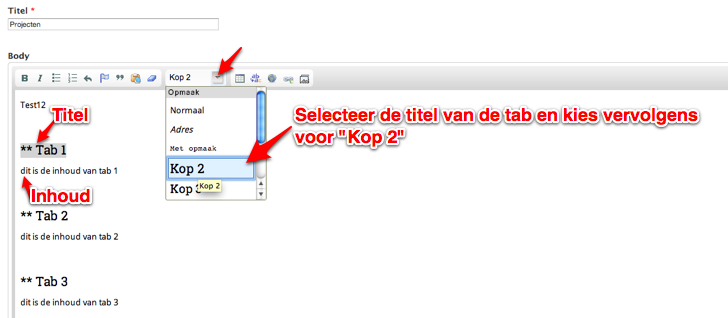
\includegraphics[width=\textwidth]{img/tabs1}
\end{center}

De onderstaande screenshot toont het resultaat.

\begin{center}
	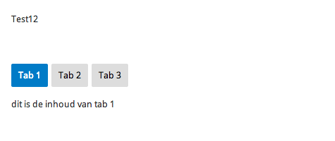
\includegraphics[width=\textwidth]{img/tabs2}
\end{center}
\subsection{Nieuwslijst}
\label{sec:nieuwslijst}
Het nieuwsgedeelte bestaat uit een lijst van de laatste vijf nieuwsberichten. Van elk bericht wordt de titel en een korte intro getoond. De titel is de link naar de detailpagina van het bericht. Onderaan de nieuwsberichten staat een link naar de nieuwsoverzichtpagina. 
\subsection{Agendalijst}
\label{sec:agendalijst}

\subsection{Grafisch element}
\label{sec:grafischelement}

\subsection{Menublok opsomming}
\label{sec:menublokopsomming}

\subsection{Menublok hierarchisch}
\label{sec:menublokhierarchisch}
Toont een hierarchische weergave van een (deel van het) menu. De getoonde onderdelen zullen afhankelijk zijn van de pagina waar de eindgebruiker op zit. Het zal maximaal twee niveau's diep tonen.
\subsection{Gerelateerde items}
\label{sec:gerelateerdeitems}

\subsection{Maps}
\label{sec:maps}
Dit blok bevat een interactieve kaartweergave van locatiegegevens gekoppeld aan een node. Deze kaart bevat zoom en pan controls.
\subsection{Downloads}
\label{sec:Downloads}
De inhoud van dit blok wordt gevuld vanuit een nodequeue. De redactie kan de inhoud van dit blok zelf samenstellen. Bestanden kunnen gekoppeld worden aan daarvoor bestemde inhoudstype. Deze nodes kunnen dan gekozen worden in een nodequeue. Het blok zal daarna een lijst tonen met de bestandsnaam, de extensie en de grootte van het gekoppelde bestand. Na het klikken op de bestandsnaam zal er een download dialoogvenster van de browser geopend worden.
\subsection{Content carrousel}
\label{sec:contentcarrousel}
Dit is een carrouselblok voor bij een node. Hier kan middels een nodequeue een selectie gemaakt worden van nodes die uitgelicht worden middels een afbeeldingencarrousel. 

Via pijlen aan de linker- en rechterkant kan door de carrousel geklikt worden. Dit kan tevens gedaan worden door met de linker- en rechterpijl op het toetsenbord.

Onder de carrousel loopt een indicator mee waardoor de eindgebruiker kan zien op welke slide hij zit. Door te klikken op een indicator zal de eindgebruiker direct naar die slide gaan. 

Wanneer de eindgebruiker met de muis over de slide hovert zal de carrousel stoppen met lopen. Er zal tevens een start- en pauzeknop aanwezig zijn waarmee de eindgebruiker op elk moment de carrousel kan starten en stoppen. Het stoppen kan ook gedaan worden via de ESC-knop op het toetsenbord.

\section{Overige functionaliteiten}
\label{sec:overigefunctionaliteiten}

\subsection{WYSIWYG}
We gebruiken een \emph{What You See Is What You Get} editor. DIt is een gebruiksvriendelijke manier van content invoeren in het CMS. De volgende opties zijn aanwezig:

\begin{itemize}
  \item Vet gedrukt
  \item Schuin
  \item Opsommings lijst
  \item Genummerde lijst 
  \item Definitie lijst
  \item Ongedaan maken
  \item Citaat
  \item Citaatblok
  \item Speciale tekens
  \item Kiezen uit opmaak
  \item Tabel
  \item Zoek en vervang
  \item Afkorting
  \item Acroniem
  \item Taal veranderen per woord
  \item Link invoegen
  \item Anker invoegen
  \item Media Invoegen
  \item Plakken speciaal
  \item Invoegen van woord
  \item Verwijderen van woord
\end{itemize}

\subsection{Fotoalbum}
Een verzameling van gegroepeerde afbeeldingen. Gebruikers kunnen afbeeldingen uploaden en voorzien van een tag. Aan het uploaden van bestanden zitten restricties van zowel grootte als omvang. De naam van het bestand zal doormiddel van \emph{transliteration} aangepast worden naar een nette naam. Hierbij worden leesteken en spaties vervangen door koppeltekens. Van de geuploade bestanden worden kleinere versies en/of uitsnedes gemaakt.

\subsection{AddThis}
Om content te kunnen delen maken we gebruik van de functionaliteit die AddThis levert. De configuratie van deze functionaliteit is eenvoudig aan te passen.

\subsection{Readspeaker}
De website zal gebruikmaken van de voorleesfunctie van Readspeaker. De functie zal aanwezig zijn op elke pagina.

\subsection{RSS}
De content die in de feeds wordt opgenomen wordt bepaald aan de hand van het veld \emph{Tonen op website} dat in een aantal content types aanwezig is. De volgorde van de content is steeds op chronologische volgorde.

\subsection{Sitemap}
Voor eindgebruikers zal er een sitemap aanwezig zijn. Deze pagina toont een overzicht van de beschikbare pagina's op de site zoals deze ingericht zijn in het menu-systeem van Drupal.

\subsection{Prikbord}
Via het content type \emph{Marketplace} kan een ingelogde gebruiker van het intranet een advertentie plaatsen. De velden titel, body en categorie kunnen daar worden ingevuld. 

\subsection{Blog}
Een ingelogde gebruiker van het intranet kan een blog maken door middel van nodes aan te maken van het content type \emph{blog}. Er komt een overzichtspagina per gebruiker waar de blog te lezen is. Er is tevens een overzichtspagina van alle blogs van alle gebruikers. Het is mogelijk om een titel, body en tags toe te voegen aan het blog.

\subsection{Responsive layout}
De website zal responsive opgezet worden. Waarbij middels verschillende breekpunten de layout van de website aangepast wordt aan de breedte van het medium. In de smalste versie van de site zullen alle kolommen (en de blokken daarbinnen) onder elkaar getoond worden. Waarbij de volgorde; linker-, midden- en rechterkolom aangehouden wordt van boven naar beneden. Op artikelpagina's zal de belangrijkste content (het artikel zelf) bovenaan getoond worden. Hier zal de volgorde van boven naar beneden dus midden-, linker- en rechterkolom.

Bij bredere versies van de site zal de middenkolom schalen en zullen de rechter- en linkerkolom dezelfde breedte houden.

\end{document}
